\documentclass[border=4pt]{standalone}
\usepackage{tikz}

\begin{document}
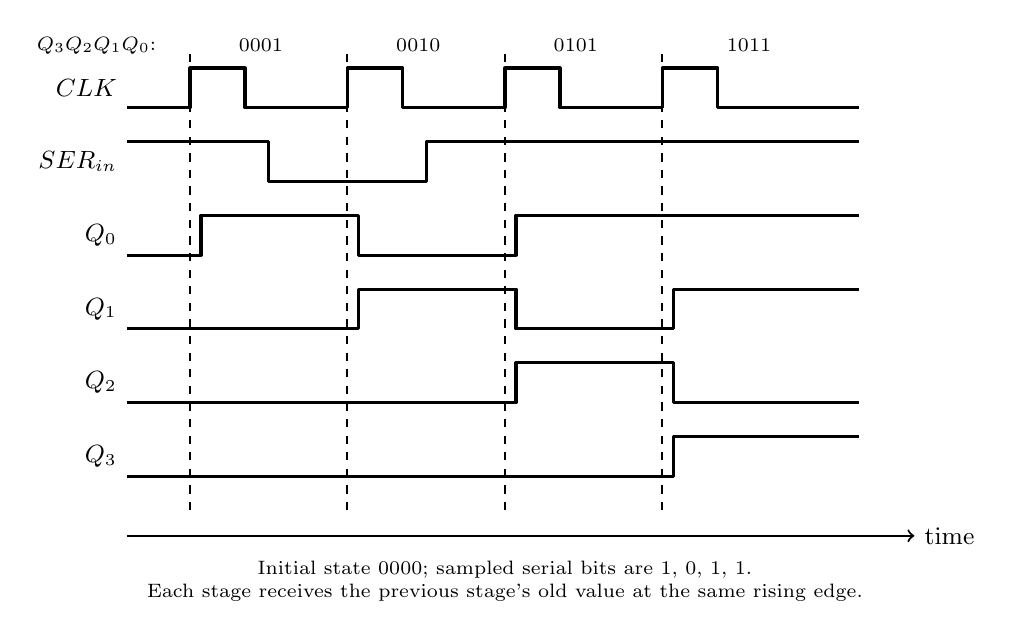
\begin{tikzpicture}[x=1cm,y=0.72cm,font=\small,line width=0.75pt,
  thick/.style={line width=1.15pt,line join=round}]
  \draw[->] (1.2,0.1) -- (11.2,0.1) node[right] {time};
  \foreach \y/\name in {8.0/$CLK$,6.7/$SER_{in}$,5.4/$Q_0$,4.1/$Q_1$,2.8/$Q_2$,1.5/$Q_3$}
    \node[left] at (1.2,\y) {\name};
  \draw[thick] (1.2,7.65) -- (2,7.65) -- (2,8.35) -- (2.7,8.35)
    -- (2.7,7.65) -- (4,7.65) -- (4,8.35) -- (4.7,8.35)
    -- (4.7,7.65) -- (6,7.65) -- (6,8.35) -- (6.7,8.35)
    -- (6.7,7.65) -- (8,7.65) -- (8,8.35) -- (8.7,8.35)
    -- (8.7,7.65) -- (10.5,7.65);
  \draw[thick] (1.2,7.05) -- (3,7.05) -- (3,6.35) -- (5,6.35)
    -- (5,7.05) -- (10.5,7.05);
  \draw[thick] (1.2,5.05) -- (2.14,5.05) -- (2.14,5.75)
    -- (4.14,5.75) -- (4.14,5.05) -- (6.14,5.05)
    -- (6.14,5.75) -- (10.5,5.75);
  \draw[thick] (1.2,3.75) -- (4.14,3.75) -- (4.14,4.45)
    -- (6.14,4.45) -- (6.14,3.75) -- (8.14,3.75)
    -- (8.14,4.45) -- (10.5,4.45);
  \draw[thick] (1.2,2.45) -- (6.14,2.45) -- (6.14,3.15)
    -- (8.14,3.15) -- (8.14,2.45) -- (10.5,2.45);
  \draw[thick] (1.2,1.15) -- (8.14,1.15) -- (8.14,1.85) -- (10.5,1.85);
  \foreach \x in {2,4,6,8} {
    \draw[dashed] (\x,0.55) -- (\x,8.7);
  }
  \node[left,font=\scriptsize] at (1.7,8.75) {$Q_3Q_2Q_1Q_0$:};
  \node[font=\scriptsize] at (2.9,8.75) {0001};
  \node[font=\scriptsize] at (4.9,8.75) {0010};
  \node[font=\scriptsize] at (6.9,8.75) {0101};
  \node[font=\scriptsize] at (9.1,8.75) {1011};
  \node[align=center,font=\scriptsize] at (6.0,-0.7)
    {Initial state 0000; sampled serial bits are 1, 0, 1, 1.\\
     Each stage receives the previous stage's old value at the same rising edge.};
\end{tikzpicture}
\end{document}
